
	
\section{Torsione}
		Ci si ponga nel caso in cui sulla faccia terminale della trave venga posto un momento torcente, questo genererà uno spostamento che non interesserà la linea d'asse, e quindi uno spostamento nullo dell'asse baricentrico: la sezione esce dal piano $xz$, il problema non è più piano. \newline 
		
		Le soluzioni esatte in forma chiusa per questo tipo di problema esistono solo per sezioni polari o per sezioni ellittiche o poligonali regolari, per altre sezioni ci si accontenta di una soluzione approssimata ma sicura. \newline 
		
		\begin{itemize}
			\item[$\rightarrow$] Per sezioni compatte la distribuzione di massa è intorno al baricentro, ed esistono alcune soluzioni esatte;
		\item[$\rightarrow$] Per sezioni in parete sottile che siano aperte o chiuse la soluzione è approssimata.
		\end{itemize} 
		
		Si ipotizzi perciò di avere una trave a sezione circolare, a simmetria polare, secondo le ipotesi che le sezioni rette ortogonali all'asse medio rimangano rette ortogonali all'asse medio, a seguito di un momento torcente ottengo una rotazione della trave, e a seguito di una rotazione è ben noto che un punto sulla sezione si muove su $x$ ed $y$.
		
\begin{figure}[H]
	\centering
	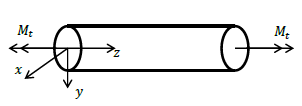
\includegraphics[width=0.5\linewidth]{immagini_5/screenshot008}
	\label{fig:screenshot008}
\end{figure}

		La rotazione della sezione intorno a $z$ sarà null'altro che proporzionale a $z$ per cui a $z=0$ la rotazione è nulla mentre a $z=l$ la rotazione è massima, l'aliquota di rotazione sarà perciò data da: 
		\[ \theta = \theta(z)= \Theta z\]
		Dove $\Theta$ è l'angolo unitario di torsione (AUT) e tiene conto della rotazione tra due facce contigue poste a distanza infinitesima.
		\[\Theta - \dfrac{\partial \theta}{\partial z}\]
		
		Per lo studio di questo problema si applica il metodo semi-inverso agli spostamenti, per cui per piccoli spostamenti, $u, v, w$ devono combaciare con la rotazione piana:

\begin{figure}[H]
	\centering
	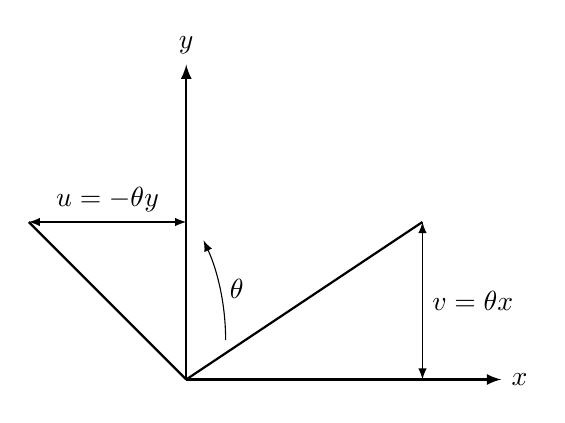
\begin{tikzpicture} [>=latex]
		%\draw [thin, help lines] (0,0) grid (5,5);
		\draw [thick, ->] (0,0) -- (4,0) node [pos = 1, right] {$x$};
		\draw [thick, ->] (0,0) -- (0,4) node [pos = 1, above] {$y$};
		\draw[->] (0.5,0.5) arc (0:25:3) node [pos = 0.5, right] {$\theta$}; 
		\draw [thick,] (0,0) -- (3,2); 
		\draw [thin, <->] (3,0) -- (3,2)  node [pos = 0.5, right] {$v = \theta x$};
		\draw [thick,] (0,0) -- (-2,2); 
		\draw [thin, <->] (0,2) -- (-2,2)  node [pos = 0.5, above] {$u = -\theta y$};
	\end{tikzpicture}
\end{figure}

		\[ \begin{cases}
			u = -\theta y = -\Theta yz \\
			v = \theta x = \Theta xz \\
			w = 0
		\end{cases}\]
		Da questi spostamenti è possibile ricavare un campo di tensioni che soddisfi l'equilibrio?
		\[ 
	\begin{cases}
		\begin{aligned}
			\varepsilon_{xx} =   \frac{\partial u_x}{\partial x} = \dfrac{1}{E}[\sigma_x - \nu(\sigma_y + \sigma_z)] = 0 \\
			\varepsilon_{yy} =   \frac{\partial u_y}{\partial y} = \dfrac{1}{E}[\sigma_y - \nu(\sigma_x + \sigma_z)] = 0 \\
			\varepsilon_{zz} =   \frac{\partial u_z}{\partial z} = \dfrac{1}{E}[\sigma_z - \nu(\sigma_x + \sigma_y)] = 0 \\
		\end{aligned}
	\end{cases} \hspace{0.2cm} \begin{cases}
		\begin{aligned}
			\gamma_{xy} =   \frac{\partial u_y}{\partial x} + \frac{\partial u_x}{\partial y} = \dfrac{1}{G} \tau_{xy} = -\Theta z + \Theta z = 0\\
			\gamma_{yz} =   \frac{\partial u_y}{\partial z} + \frac{\partial u_z}{\partial y} = \dfrac{1}{G} \tau_{xz} = -\Theta y \\
			\gamma_{zx} =   \frac{\partial u_z}{\partial x} + \frac{\partial u_x}{\partial z} = \dfrac{1}{G} \tau_{yz} = \Theta x \\
		\end{aligned}
	\end{cases}
		\]
		Le dilatazione sono nulle, così come le distorsioni $\gamma_{xy}$, ma lo stesso non si può dire per le distorsioni $\gamma_{zx}$ e $\gamma_{yz}$, entrambe non nulle. \newline 
	
		Il che si traduce nell'avere la completa assenza di azioni normali, queste soppiantate dalle sole azioni tangenziali, la torsione genera soltanto tensioni di tipo tangenziale: 
		\[ \tau_{xz} = -G\Theta y \hspace{1cm} \tau_{yz} = G\Theta x\]
		Il tensore delle tensioni diviene così: 
	 	\[ \left[ \begin{array}{ccc}
		0 & 0 & -G\Theta y \\
		0 & 0 & G\Theta x \\
		-G\Theta y & G\Theta x & 0
		\end{array}\right] \]
		Si verifichi adesso il problema di De Saint Venant attraverso gli equilibri. 
		
		Per gli equilibri interni le condizioni indefinite di equilibrio risultano immediatamente soddisfatte, col risultato che il campo di tensioni risulta piano (sempre per quel discorso che $\det[\sigma]\equiv\Rightarrow\exists$ almeno due soluzioni) 
		\[
		\begin{cases}
			\begin{aligned}
				\frac{\partial \tau_{zx}}{\partial z} & =0 \\
				
				\frac{\partial \tau_{zy}}{\partial z} & =0 \\
				
				\frac{\partial \tau_{xz}}{\partial x} + \frac{\partial \tau_{yz}}{\partial y} + \frac{\partial\sigma_z}{\partial z} & =0 \\
			\end{aligned}
		\end{cases}
		\]
		Le condizioni al contorno si trasformano in:
		\[ \tau_{xz}n_x + \tau_{yz}n_y = 0\]
		Si è dimostrato in questo modo come il vettore tensione sia ortogonale alla normale
		della giacitura coincidente la superficie tangente al
		bordo della sezione nel punto in esame, perché banalmente, se $n_x, n_y$ sono co coseni direttori della normale e il vettore tensione si può scrivere secondo le sue componenti $\vec{\tau}_z = (\tau_{xz}\hat{i} +  \tau_{yz}\hat{j})$, allora:
		\[\vec{\tau}_z \cdot \hat{n} = 0\]
		Nel caso specifico di sezione circolare, si può scrivere questa relazioni in termini di raggio, d'altronde è ben noto che in una sezione siffatta la normale è radiale, per cui: 
		\[\hat{n} = \vec{R} = x\hat{i} + y\hat{j}\]
		A allora varrà ugualmente che la direzione del vettore tensione sarà sempre ortogonale al vettore posizione, che in una sezione circolare corrisponde ad una variabile radiale:
		\[\vec{\tau}_z \cdot \vec{R} = 0 \Rightarrow \tau_{xz}x +  \tau_{yz}y = 0 \Rightarrow -G\Theta yx + G\Theta xy =0 \]
		\[ G\Theta yx = G\Theta xy \]
		Si è così al cospetto della soluzione esatta. 
		
		Tutti
		punti sullo stesso diametro hanno un vettore tensione con direzione costante e modulo
		proporzionale alla distanza dall’asse di rotazione. 
		
		\paragraph{Osservazione} \mbox{} \\ 		
			$\vec{\tau}_z$ è tangente al bordo, ma in una sezione circolare questo significa che è sempre ortogonale al raggio: avrà sempre direzione circonferenziale rispetto al sistema di riferimento, ovvero esiste una linea di flusso di $\tau$ che si chiude lungo tutto il bordo, è una circonferenza, un luogo di punti caratterizzato dalla stessa tensione, dalla stessa intensità del vettore tensione, in cui è sempre uniforme in modulo ma non in direzione e verso, queste dettate dalla tangenza della linea di flusso stessa.
			
\begin{figure}[H]
	\centering
	\begin{tikzpicture} [>=latex]
		%\draw [thin, help lines] (0,0) grid (5,5);
		\draw (2.5,2.5) circle (2.5 and 2.5);
		\draw[->] (2.5,2.5) -- (3.5,2.5) node [pos=1, right] {$x$};
		\draw[->] (2.5,2.5) -- (2.5,3.5) node [pos=1, above] {$y$};
		%\draw (0.75,0.75) -- (4.25,4.25);
		%\draw [rotate around={30:(2.5,2.5)}] (0.75,0.75) -- (4.25,4.25);
		\draw[pattern=vertical lines] (4.25,4.25) -- (3.14, 4.91) -- (2.5,2.5) -- (4.25,4.25);
		\draw[pattern=vertical lines] (0.75,0.75) -- (1.89, 0.09) -- (2.5,2.5) -- (0.75,0.75);
		
		\foreach \angle in {0, 30, 60, 90, 120, 150, 180, 210, 240, 270, 300, 330}
		{
			\pgfmathsetmacro{\x}{2.5 + 2.5 * cos(\angle)}
			\pgfmathsetmacro{\y}{2.5 + 2.5 * sin(\angle)}
			\draw[->] (\x, \y) -- ++({-sin(\angle)}, {cos(\angle)});
		}
	\end{tikzpicture}
\end{figure}

			Le linee di flusso del vettore tensione sono circonferenze
			concentriche con la circonferenza che individua il bordo
			della sezione retta.
			
			Il diagramma in esame inoltre fornisce la vera rappresentazione del vettore tensione! Col momento torcente, a differenza del momento flettente, so rappresentando direzione, verso, e intensità sullo stesso diagramma.
			\[ |\vec{\tau}_z| = \sqrt{\tau^2_{xz} + \tau^2_{yz}} = G\Theta\sqrt{x^2 + y^2} = G\Theta r\]
			$\vec{\tau}_z$ è in questo modo linearmente dipendente dalla quota radiale, oltre che essere ortogonale a $\vec{R}$. \newline 
			
			Il problema però è che ancora non so determinare l'angolo unitario di torsione $\Theta$. 
			
			Mi corrono in soccorso le caratteristiche della sollecitazione, di cui però si è già ricavato le tensioni, si vede subito che le uniche caratteristiche che interessano la trattazione sono: 
			caratteristiche della sollecitazione sulla $S_l$ perciò saranno:
			\[\begin{matrix}
				\begin{aligned}
					T_x = \int_A \tau_{zx}dA = -G\Theta\int_AydA = -G\Theta S_x = 0 &  \\
					T_y = \int_A \tau_{zy}dA = G\Theta\int_AxdA = G\Theta S_y =0 \hspace{1cm} &  M_z = \int_A (\tau_{zy}x -\tau_{zx}y)dA
				\end{aligned}	
			\end{matrix}\]
			Dove gli $S_i$ sono nulli per la classica ipotesi di sistema riferimento baricentrale, il momento $M_z$ per rispettare l'equilibrio, dovrà proprio essere uguale al momento torcente:
			\[ M_z = M_t = \int_A (\tau_{zy}x -\tau_{zx}y)dA = G\Theta\int_Ax^2dA + G\Theta\int_Ay^2dA = G\Theta\int_A(x^2 + y^2)dA = G\Theta I_z \]
			Dove si è identificato con $I_z$ il momento d'inerzia polare, rispetto all'asse ortogonale alla sezione stessa, somma dei contributi di momento d'inerzia su $x$ ed $y$. \newline
			
			Da quest'ultima relazione so così finalmente trovarmi l'angolo $\Theta$: 
			\[ \Theta = \dfrac{M_t}{GI_z}\]
			In cui $GI_z$ è il modulo di rigidezza torsionale. \newline 
			
			Quest'angolo si può immediatamente sostituire negli spostamenti e nelle tensioni ottenendo: 
			\[ \begin{cases}
				u = -\Theta yz = -\dfrac{M_t}{GI_z}yz \\
				v =  \Theta xz = \dfrac{M_t}{GI_z} xz\\
				w = 0
			\end{cases} \hspace{0.3cm} \tau_{xz} = -G\Theta y = -\dfrac{M_t}{I_z}y  \hspace{0.3cm} \tau_{yz} = G\Theta x = \dfrac{M_t}{I_z}x\]
			La rotazione infine sarà data da quella della faccia finale meno quella della faccia iniziale, se la rotazione era definita come $\theta = \Theta z$ e se per ipotesi la rotazione sulla faccia iniziale era data nulla, si ha: 
			\[\Delta\theta = \theta(L) - \theta(0) = \theta(L) = \dfrac{M_t}{GI_z}L\]
			Infine, matematicamente l'inerzia polare per una sezione circolare può essere scritta come: 
			\[ I_z = \int_A r^2dA = \dfrac{\pi R^4}{2}\]
			Così, se nella sua forma finale $|\vec{\tau}_z| = G\Theta r$, si potrà scrivere:
			\[ \boxed{\tau_z = \dfrac{M_t}{GI_z}r = \dfrac{2M_t}{\pi R^4}r} \]
			\begin{figure}[H]
				\centering
				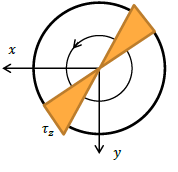
\includegraphics[width=0.2\linewidth]{immagini_5/screenshot002}
				\label{fig:screenshot002}
			\end{figure}
			
			Si vede immediatamente che le tensioni massime si genereranno al bordo esterno della sezione retta.\newline 
			
			Tale modello sarà perfettamente riproducibile (a meno di sezione assialsimmetrica) anche al caso di sezioni circolari cave, in cui l’unico aspetto
			modificato risulta il valore del momento di inerzia polare, ma valendo i principi booleani di somma e sottrazione delle aree si possono senza problemi combinare le rispettive inerzie delle sezioni: 
			\[ \boxed{\tau_z = \dfrac{2M_t}{\pi (R_{ext}^4-R_{int}^4)}r} \]
			
\begin{figure}[H]
	\centering
	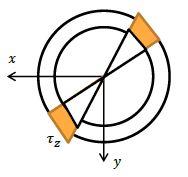
\includegraphics[width=0.2\linewidth]{immagini_5/screenshot001}
	\label{fig:screenshot001}
\end{figure}


			Quando lo spessore della parete diminuisce, la differenza tra il vettore tensione al raggio esterno e quello al raggio interno diviene decisamente trascurabile, si perviene in questo modo a soluzioni ancor più semplificate che prevederanno una costanza di $\tau$ lungo tutto lo spessore. \newpage

\subsection{Sezione generica}
		La soluzione precedente non è però applicabile ad una sezione generica. 
\begin{figure}[H]
	\centering
	\label{fig:screenshot003}
	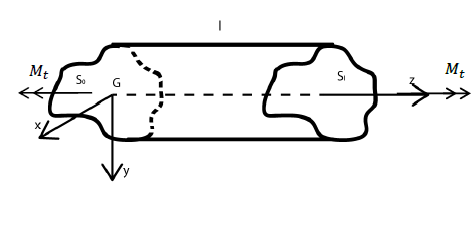
\includegraphics[width=0.5\linewidth]{immagini_5/screenshot003}
\end{figure}
		Ad esempio, una $\tau$ circonferenziale non soddisfa più le condizioni al contorno di ortogonalità in tutti i punti del bordo, è dunque necessario cercare una nuova soluzione o modificare quella precedente.
		
		Si mettono dei paletti ad $u$ e $v$, questi sono intoccabili e garantiscono che la sezione ruoti in modo uniforme senza separazione di materiale, rimuovo allora l'ipotesi che le sezioni piane rimangano piane. 
		
		Attribuisco così a $w$ una funzione $\omega(x,y)$, dipendente dalla specifica forma della sezione, che mi dirà lo spostamento in $z$ essere concesso. 
		
		Tale spostamento lo si proporzionerà all'angolo unitario di torsione e lo si definisce per ipotesi costante in $z$: tutte le sezioni si sposteranno della stessa quantità, a seguito della torsione le fibre si muoveranno in direzione $z$ ognuna in modo differenziato.
		
		\textbf{NB:} Le fibre si spostano soltanto in direzione $z$, non si dilatano, la forma della sezione rimarrà la stessa, è come si si lasciasse un'impronta su di una faccia estremale di cui si troverà il negativo sulla faccia estremale opposta, l'impronta è proprio la funzione ingobbamento, che si ritroverà esattamente identica in tutte le sezioni della trave, fino alla faccia frontale.  		
		\[ \varepsilon_{zz} = \dfrac{\partial w}{\partial z} = 0 \Rightarrow \begin{cases}
			u = -\Theta yz  \\
			v =  \Theta xz  \\
			w = \Theta \omega(x,y)
		\end{cases} \]
		Avendo rimosso così la simmetria polare, ci si aspetta
		che la sezione trasversale presenti un \textbf{ingobbamento $\omega(x,y)$},
		costante per tutte le sezioni.\newline 
		
		Come definisco le tensioni? 
		\[ 
		\begin{cases}
			\begin{aligned}
				\varepsilon_{xx} =   \frac{\partial u_x}{\partial x} = 0 \\
				\varepsilon_{yy} =   \frac{\partial u_y}{\partial y} = 0 \\
				\varepsilon_{zz} =   \frac{\partial u_z}{\partial z} = 0 \\
			\end{aligned}
		\end{cases} \hspace{0.2cm} \begin{cases}
			\begin{aligned}
				\gamma_{xy} =   \frac{\partial u_y}{\partial x} + \frac{\partial u_x}{\partial y} = -\Theta z + \Theta z = 0\\
				\gamma_{yz} =   \frac{\partial u_y}{\partial z} + \frac{\partial u_z}{\partial y} = \dfrac{1}{G} \tau_{xz} = \Theta \left(\dfrac{\partial \omega}{\partial x}-y\right) \\
				\gamma_{zx} =   \frac{\partial u_z}{\partial x} + \frac{\partial u_x}{\partial z} = \dfrac{1}{G} \tau_{yz} = \Theta \left(\dfrac{\partial \omega}{\partial y} + x\right)\\
			\end{aligned}
		\end{cases}
		\]
		Lo stato tensionale deve rispettare l’equilibrio interno al volume:
		\[
		\begin{cases}
			\begin{aligned}
				\frac{\partial \tau_{zx}}{\partial z} & =0 \\
				
				\frac{\partial \tau_{zy}}{\partial z} & =0 \\
				
				\frac{\partial \tau_{xz}}{\partial x} + \frac{\partial \tau_{yz}}{\partial y} + \frac{\partial\sigma_z}{\partial z} & = \frac{\partial \tau_{xz}}{\partial x} + \frac{\partial \tau_{yz}}{\partial y} = \vec{\nabla}\cdot\vec{\tau}_z = 0 \\
			\end{aligned}
		\end{cases}
		\]
		Quello che si ottiene e che, affinché venga verificata l'ultima equazione, deve valere:
		\[ \vec{\nabla}\cdot\vec{\tau}_z = 0 \]
		\[G\Theta\left(\dfrac{\partial^2 \omega}{\partial y^2} + \dfrac{\partial^2 \omega}{\partial x^2} \right)= 0\]
		Vera se e solo se:
		\[ \boxed{\dfrac{\partial^2 \omega}{\partial y^2} + \dfrac{\partial^2 \omega}{\partial x^2} = 0} \]
		Ovvero se la funzione ingobbamento è una funzione armonica. \newline 
		
		Quello che cambia ora è che l'equilibrio non è più identicamente dimostrato dalla semplice sostituzione delle $\tau$, anzi, è funzione dell'ingobbamento stesso! \newline 
		
		Si verifichino ora le condizioni al contorno che per la torsione abbiamo imparato a sintetizzare come: 
		\[\vec{\tau}_z \cdot \hat{n} = 0\]
		Questa vera se e solo se: 
		\[ G\Theta \left[\left(\dfrac{\partial \omega}{\partial x} - y\right)n_x + \left(\dfrac{\partial \omega}{\partial y} +x\right)n_y\right] = 0\]
		\[ \dfrac{\partial \omega}{\partial x}n_x + \dfrac{\partial \omega}{\partial y}n_y - yn_x  + xn_y = 0\]
		In forma vettoriale $n_x, n_y$ identificano i coseni direttori della normale alla superficie, $,x,y$ identificano il vettore radiale, mentre $ -n_y, n_x$ identificano il vettore tangenziale.
		
\begin{figure}[H]
	\centering
	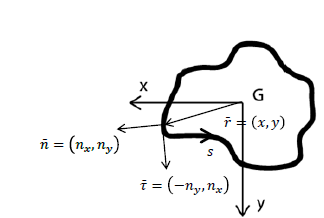
\includegraphics[width=0.5\linewidth]{immagini_5/screenshot004}
	\label{fig:screenshot004}
\end{figure}
		
		\[ \vec{\nabla}\omega \cdot \hat{n} - \hat{r} \cdot \hat{t} = 0\]
		Si sfrutti ora la proprietà del gradiente per il quale se si cambiano le coppie di assi rispetto alle quali si effettuano le derivate parziali, il valore del gradiente non cambia, per cui:
		\[ \left(\dfrac{\partial \omega}{\partial t}, \dfrac{\partial \omega}{\partial n} \right)\cdot \hat{n} - \hat{r} \cdot \hat{t} = 0\]
		Vera se e solo se: 
		\[ \boxed{\dfrac{\partial \omega}{\partial n} = \hat{r} \cdot \hat{t}}\]
		La determinazione della funzione di
		ingobbamento prende il nome di problema di Neumann, che si risolve in forma chiusa per poche sezioni. \newline 
		
		Si dimostri adesso, tramite le caratteristiche della sollecitazione, che tale condizione al contorno appena trovata sia verificata. 
		\[ \begin{split} T_x & = \int_A \tau_{zx}dA =  \int_A\underbrace{\left(\dfrac{\partial}{\partial x}(x\tau_{zx}) -x\dfrac{\partial\tau_{zx}}{\partial x}\right)}_\text{$\dfrac{\partial}{\partial x}(x\tau_{zx}) = 1\tau_{zx} +x\dfrac{\partial\tau_{zx}}{\partial x}$}dA = \\
		& = \int_A \left(\dfrac{\partial}{\partial x}(x\tau_{zx}) -x\left(\dfrac{\partial\tau_{zx}}{\partial x} \underbrace{+ \dfrac{\partial\tau_{zy}}{\partial y} - \dfrac{\partial\tau_{zy}}{\partial y}}_\text{Sommo e Sottraggo}\right)\right) = \\
		& = \int_A\left(\dfrac{\partial}{\partial x }(x\tau_{zx}) + \dfrac{\partial}{\partial y}(x\tau_{zy})\right) = \\ 
		& = \int_{\partial A} x(\tau_{zx}n_x + \tau_{zy}n_y)ds = \int_{\partial A} x(\vec{\tau}\cdot \hat{n})ds = 0	\end{split}\]
		Dove ci si è ricordati che $\dfrac{\partial\tau_{zx}}{\partial x} + \dfrac{\partial\tau_{zy}}{\partial y} =0$. \newline 
		
		Similmente varrà: 
		\[ T_x = \int_A \tau_{zy}dA = 0 \]	
		
		Per il momento invece, so che è pari al momento torcente imposto: 
		\[ \begin{split}
			M_z & = M_t = \int_A (\tau_{zy}x -\tau_{zx}y)dA = G\Theta\int_A \left(x^2 + y^2 + x\dfrac{\partial\omega}{\partial y} - y\dfrac{\partial\omega}{\partial x}\right)dA = \\
			& = G\Theta \left[ I_z + \int_A \left(x\dfrac{\partial\omega}{\partial y} - y\dfrac{\partial\omega}{\partial x}\right)dA \right] = \\
			& = G\Theta J_t
		\end{split}\]
		Con $J_t$ inerzia torsionale.
		
		L'angolo incognito diviene così funzione dell'inerzia torsionale, funzione essa di un integrale geometrico dell'ingobbamento: 
		\[ \Theta = \dfrac{M_t}{GJ_t}\]
		Ci si riconduce così ai casi in cui $\omega = 0$ e l'inerzia torsionale coincide con l'inerzia polare e la sezione e circolare e nel caso generico dove $\omega\neq 0$ ed è necessario calcolare la funzione ingobbamento attraverso il problema di Neumann. \newline 
		
		Si ottiene così, per spostamenti e tensioni: 
			\[ \begin{cases}
			u = -\Theta yz = -\dfrac{M_t}{GJ_t}yz \\
			v =  \Theta xz = \dfrac{M_t}{GJ_t}xz\\
			w = \dfrac{M_t}{GJ_t}\omega(x,y)
		\end{cases} \hspace{1cm} \begin{aligned}
		\tau_{xz} &= G\Theta \left(\dfrac{\partial \omega}{\partial x}-y\right) =\dfrac{M_t}{J_t}  \left(\dfrac{\partial \omega}{\partial x}-y\right) \\
		\tau_{yz} &= G \Theta \left(\dfrac{\partial \omega}{\partial y} + x\right) = \dfrac{M_t}{J_t} \left(\dfrac{\partial \omega}{\partial y} + x\right)
	\end{aligned}\]
	Non importa più per quale asse o punto applico il momento di torsione ora, può essere anche non baricentrico, lo stato tensionale sarà del tutto identico a quello ricavato secondo l'asse baricentrico. 
	
	Applicando il momento torcente per un asse parallelo a $z$ e non baricentrico, le tensioni che si ricavano sono esattamente identiche a quelle ricavate applicando lo stesso momento intorno all'asse $z$ baricentrico. \newline 
	
	La funzione ingobbamento si trova solo per determinate sezioni, le cui tensioni sono rispettivamente: 
	\[\begin{array}{cc}
		\text{Sezione ellittica} & \text{Sezione triangolare} \\ 
		\tau_{xz} = -\dfrac{2M_t}{\pi pq^3}y; \tau_{yz} = \dfrac{2M_t}{\pi pq^3}x  & \tau_{z, max} = \dfrac{M_t}{0.2Ad}  
	\end{array}\]
   \[\begin{array}{ccc}
   	\text{Sezione quadrata} & \text{Sezione esagonale} & \text{Sezione ottagonale} \\
   	\tau_{z, max} = \dfrac{M_t}{0.208Ad} & \tau_{z, max} = \dfrac{M_t}{0.217Ad} & \tau_{z, max} = \dfrac{M_t}{0.223Ad}
   \end{array}\]
			Con $p,q$ semiassi dell'ellisse e $d$ diametro del cerchio iscritto.  
			
\subsubsection{Considerazioni}
			Se è vero che non si può trovare la soluzione in forma chiusa, è anche vero che in qualche modo le tensioni e le sollecitazioni andranno ricavate. 
			
			L'ingobbamento porta con se due fatti notevoli, il primo deriva dall'equazione dell'equilibrio interno $\vec{\nabla} \cdot \vec{\tau} = 0$ mentre il secondo dall'equilibrio al contorno $\vec{\tau} \cdot \hat{n}=0$, tutto ciò si può riassumere dicendo che le linee di flusso appartenenti ad una sezione qualunque sono chiuse, con il notevole risultato di avere un campo di tensione solenoidale: esisterà un luogo dei punti descritto da una curva chiusa caratterizzata da tensioni in modulo identico e direzione tangenziale rispetto a tale curva, con verso imposto dal momento torcente.\newline

			 Inoltre, girando, il campo mi assicura un rotore diverso da zero, costante sul volume e costante rispetto a $z$:
			 \[\vec{\nabla} \times \vec{\tau} = G\Theta \left[\left(\dfrac{\partial^2\omega}{\partial y \partial x} + 1\right) - \left(\dfrac{\partial^2\omega}{\partial x \partial y} - 1\right)\right]\hat{k} = 2G\Theta\hat{k}\]
			 Dove è proprio Schwarz ad assicurarmi che le derivate incrociate sono uguali perché cambiando ordine di derivazione il risultato non cambia. \newline 
			 
			 I vettori di flusso si comportano come i vettori di velocità in un fluido in rotazione, dove c'è restrizione le linee di flusso si avvicinano provocando una tensione tangenziale maggiore, e viceversa, dove c'è allargamento le linee di flusso si diradano e la tensione diminuisce. \newline 
			 
			 Inoltre nelle sezioni
			 sottili chiuse le tensioni tangenziali sono parallele alla linea media e distribuite
			 uniformemente lungo lo spessore mentre nelle sezioni sottili aperte sono parallele alla linea media e variano
			 linearmente lungo lo spessore (valori massimi ai bordi e nulli sulla linea media). 
			 
\subsection{ Sezione rettangolare sottile aperta}
			 \textit{Una sezione è aperta se la sua linea media non si chiude. }\newline
			 
			 La sezione rettangolare sottile è un primo esempio di forte approssimazione data da un forte errore di equilibrio, che però non è tuttavia così importante ai fini delle sollecitazione massime.  
			 
\begin{figure}[H]
	\centering
	\label{fig:screenshot005}
	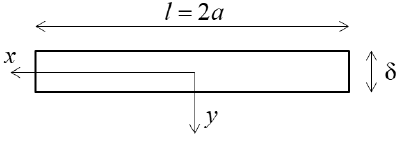
\includegraphics[width=0.5\linewidth]{immagini_5/screenshot005}
\end{figure}

		
			 Nella sezione circolare il vettore $\tau$ era sempre parallelo alla parete. Se lo spessore lo permetteva, un'altra linea di flusso più interna prevedeva anch'essa vettori paralleli a quella esterna di modulo identico, il che stava a significare un vettore $\tau$ costate lungo tutto lo spessore.  
			 
			 \begin{figure}[H]
			 	\centering
			 	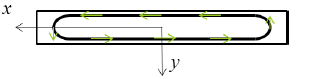
\includegraphics[width=0.5\linewidth]{immagini_5/screenshot006}
			 	\label{fig:screenshot006}
			 \end{figure}
			 
			 Nel caso di sezioni sottili aperte invece, al $\tau$ sono associate alla stessa quota, sì gli stessi valori, ma opposti, col risultato di un andamento dipendente dallo spessore. Inoltre, come si vede, a parte nelle sezioni estremali, le tensioni sono sempre parallele ai lati lunghi della sezione, per cui a meno di quelle singolarità posso considerare senza - forse - commettere troppi errori:
			 \[ \tau_{zx} = \tau_z\]
			 Con un andamento che dipende da $y$, come detto. 
			 
\begin{figure}[H]
	\centering
	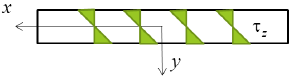
\includegraphics[width=0.5\linewidth]{immagini_5/screenshot007}
	\label{fig:screenshot007}
\end{figure}

			Se esistono soluzioni di Neumann per una trave quadrata allora esisteranno anche per travi rettangolari, queste sono date da:
			\begin{equation} 
				\label{taumax}
				\tau_{z, max} = \dfrac{M_t}{\dfrac{1}{3}l\delta^2} 
			\end{equation}
			\[ \tau_{xz} = -2\dfrac{M_t}{J_t}y \hspace{0.5cm} J_t = \dfrac{1}{3}l\delta^2 \hspace{1cm} \tau_{zx, max} = \dfrac{M_t}{J_t}\delta \hspace{1cm} \Theta = \dfrac{M_t}{GJ_t} \]
			È questa una soluzione che soddisfa tutte le condizioni? No, è approssimata, tale approssimazione si nota dall'equilibrio delle sollecitazioni, integro il contributo della tensione dovuto alla distribuzione:
			\[ M_z = \int_A(-\tau_{zx}y)dA = \int_A2\dfrac{M_t}{J_t}y^2dA =2\dfrac{M_t}{J_t}l\int_{-\delta/2}^{\delta/2}y^2dy = \dfrac{1}{6}\dfrac{M_t}{J_t}l\delta^3 = \dfrac{M_t}{2}  \]
			Il momento derivato dalle $\tau_{zx}$ così ipotizzato è pari soltanto alla metà del momento torcente applicato, non sta in equilibrio, non è verificata l'uguaglianza; le tensioni estremali che si erano trascurate, seppur agiscano solo agli estremi, danno una risultante con un braccio importante provocando una notevole coppia torcente, da sole quelle tensioni contribuiscono come metà del momento torcente. 
			
\begin{figure} [H]
	\centering
	\begin{tikzpicture} [>=latex]
	%\draw [thin, help lines] (0,0) grid (5,5);
	\draw[thick] (0,0) rectangle (4, 1);
	\draw[pattern = north west lines] (0,0) -- (0,1) -- (0.5, 0.5) -- (0,0);
	\draw[pattern = north west lines] (4,0) -- (4,1) -- (3.5, 0.5) -- (4,0);
	\draw[<->] (2,0) -- (2,1) node [pos = 0.5, right] {$\delta$};
	\draw[->] (0,0) -- (0, -1) node [pos = 1, left] {$\tau_{zy}$};		
	\draw[->] (4,1) -- (4, 2) node [pos = 1, right] {$\tau_{zy}$};
\end{tikzpicture}
\end{figure}

			Per avere equilibrio dovranno contribuire allora anche le $\tau_{yz}$, queste ricavabili a posteriori.

			Come quantifico queste forze? Approssimo una $\tau_{yz}$ costante che agisca su quell'area così si trova la forza.			
			\[\underset{forza}{\tau_{yz} \cdot \underset{area}{\dfrac{\delta \cdot \delta/2}{2}}} \cdot \underset{braccio}{l} = \dfrac{M_t}{2}  \]
			Giungendo a:
			\[  \tau_{yz} = \dfrac{2M_t}{l\delta^2} \]
			Il contributo delle $\tau_{yz}$ è assai minore del contributo delle $\tau_{zx, max}$ (\ref{taumax}). \newline
			
			Se è vero che trascurando gli estremi sto commettendo un errore di equilibrio rispetto alla sollecitazioni, è anche vero che, se voglio trovare la tensione massima agente nella sezioni, con questo approccio si trova. Agli estremi comunque si verificheranno effetti di bordo, ma per una verifica atta a trovare la porzione di trave più sollecitata, basta ricavare la $\tau_{zx, max}$: stimo l'azione locale, la più importante. \newline 
			
			Inoltre, a maggior ragione, laddove è massima la $\tau_{zx}$ è nulla la $\tau_{yz}$: sulla frontiera, per rispettare le condizioni al contorno non si possono avere componenti in direzione $y$, $\tau_z$ è per forza orientato come $x$, e allora a quel punto la soluzione risulterà localmente esatta!
			
			Non sarà invece esatto dire che la soluzione sarà quella per tutta la lunghezza.  
			
\subsection{Sezione sottile aperta monoconnessa}
\begin{figure}[H]
	\centering
	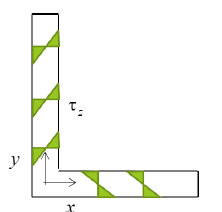
\includegraphics[width=0.3\linewidth]{immagini_5/screenshot010}
	\label{fig:screenshot010}
\end{figure}

			Sotto la validità delle proprietà booleane, mi posso ricondurre ad una somma di sezioni rettangolari, considerando l'inerzia totale come somma delle inerzie, per cui: 
			\[J_t = \dfrac{1}{3}\sum_il_i\delta^3_i\]
			\[ \tau = \dfrac{M_t}{J_t}\delta\]
			La tensione massima si valuterà invece tratto per tratto e nella formula ci andrà al denominatore l'inerzia totale dell'intera sezione, mentre al numeratore il valore dello spessore in quel tratto, per spessori variabili si tornerà invece alle formulazioni con $y$ esplicito: 
			\[ \tau_{xz} = -2\dfrac{M_t}{J_t}y \]
			Notare che una maggiore tensione si troverà su una sezione del tratto più spesso, perché in fin dei conti, il valore $\dfrac{M_t}{J_t}$ è null'altro che il coefficiente angolare di una retta che ha la stessa pendenza su tutta la sezione. \newline 
			
			Alcune sezioni notevoli:
			\[\begin{array}{ccc}
				\text{Sezione L} & \text{Sezione tubolare aperta} \\
				J_t = \dfrac{1}{3}(b+h)\delta^3 \hspace{0.2cm} \tau_{z,max} =\dfrac{3M_t}{(b+h)\delta^3}  & J_t = \dfrac{1}{3}(2\pi R)\delta^3\hspace{0.2cm}  \tau_{z,max} =\dfrac{3M_t}{(2\pi R)\delta^3}   
			\end{array}\]
			\[ \begin{array}{c}
				\text{Sezione C} \\
				J_t = \dfrac{1}{3}(2b+h)\delta^3 \hspace{0.2cm}  \tau_{z,max} =\dfrac{3M_t}{(2b+h)\delta^3} 
			\end{array}\]
		
\subsection{Sezione sottile aperta pluriconnessa}
		\textit{La linea media non forma un percorso chiusa ma si biforca.}  
		\begin{figure}[H]
			\centering
			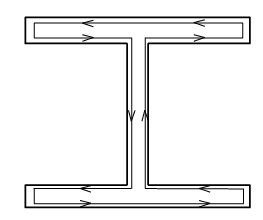
\includegraphics[width=0.3\linewidth]{immagini_5/screenshot011}
			\label{fig:screenshot011}
		\end{figure}
		
		Pratico lo stesso approccio appena portato a termine:
		\begin{enumerate}
			\item Si suddivide la sezione in porzione rettangolari \( J_{t,i} = \dfrac{1}{3}l_i\delta^3_i \)
			\item Si ripartisce il momento torcente tra i rettangoli \( \tau_{max,i} = \dfrac{M_{t,i}}{J_{t,i}}\delta_i\)
			\item Si ricavano le tensioni sul singolo rettangolo
		\end{enumerate}
		L’inerzia torsionale della sezione è data dalla somma delle inerzie dei
		singoli rettangoli:
		\[ M_t = \sum_i G\Theta J_{t,i} = G\Theta \sum_i J_{t,i} = G\Theta J_t\]
		\[ J_t = \sum_i J_{t,i} \]
		Ogni rettangolo è sottoposto ad una frazione del momento torcente
		proporzionale alla propria inerzia torsionale, ogni rettangolo si prende la sua quota di momento torcente in base a quanto è rigido:
		\[ M_{t,i} = M_t\dfrac{J_{t,i}}{J_{t}} \]
		Le tensioni tangenziali massime sono funzione dello spessore del
		rettangolo: massime nel rettangolo con spessore maggiore.
		\[ \tau_{max,i} = \dfrac{M_{t,i}}{J_{t,i}}\delta_i = \dfrac{M_t}{J_t}\delta_i \]
		Nelle sezioni pluriconnesse non è importante andare a capire quanto vale il momento torcente o la sua aliquota sul singolo tratto rettangolare, l'importante è conoscere lo spessore di ciascun termine, alla fine l'andamento a farfalla ha sempre la stessa pendenza su ciascun ramo: a spessori maggiori corrisponderanno sempre tensioni maggiori e si localizzeranno sull'estradosso. 	 
			
\subsection{Sezione cava a parete sottile}
		Si consideri una trave la cui sezione retta è caratterizzata da una linea media che sia una curva sufficientemente
		regolare nel piano o equivalentemente formata da archi di curva regolari. 
		
		Sotto le seguenti ipotesi:
		\begin{itemize}
			\item Spessore piccolo rispetto alla lunghezza della linea media \(\dfrac{\delta(s)}{a}<<1\)
			\item Funzione dello spessore continua \( a = \int_{l_m}ds\)
			\item Curvatura della linea media  piccola \(\dfrac{\delta(s)}{R}<<1\)
			\item Per sezioni generate da spezzate veridicità di tali condizioni a tratti  \( \left|\dfrac{d\delta(s)}{d}\right|<<1 \)
		\end{itemize}
		Vale quanto detto fin'ora, lungo lo spessore $\tau$ sarà costante, a maggior ragione se la sezione si chiude su se stessa.
		
\begin{figure}[H]
	\centering
	\label{fig:screenshot012}
	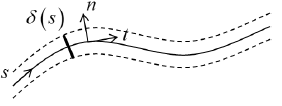
\includegraphics[width=0.5\linewidth]{immagini_5/screenshot012}
\end{figure}
		
		L’ipotesi di sottigliezza implica che le normali al bordo esterno a quello interno e alla linea media siano coincidenti
		in direzione: le tensioni tangenziali devono essere necessariamente orientate come $\hat{t}$ per rispettare l’equilibrio al
		contorno. \newline 
		
		Si immagini di tagliare la sezione chiusa con due code generiche, l'equilibrio a traslazione vedrà l'instaurarsi degli sforzi tangenziale uguali e contrari \newline \(\tau_1\delta_1\cdot 1 = \tau_2\delta_2\cdot 1 \), valendo a dire questo che la distribuzione delle tensioni $\tau$ genera un flusso di tensione costante:
		\[\tau\delta = q \Rightarrow \tau = \dfrac{q}{\delta}\]
\begin{figure}[H]
	\begin{center}
		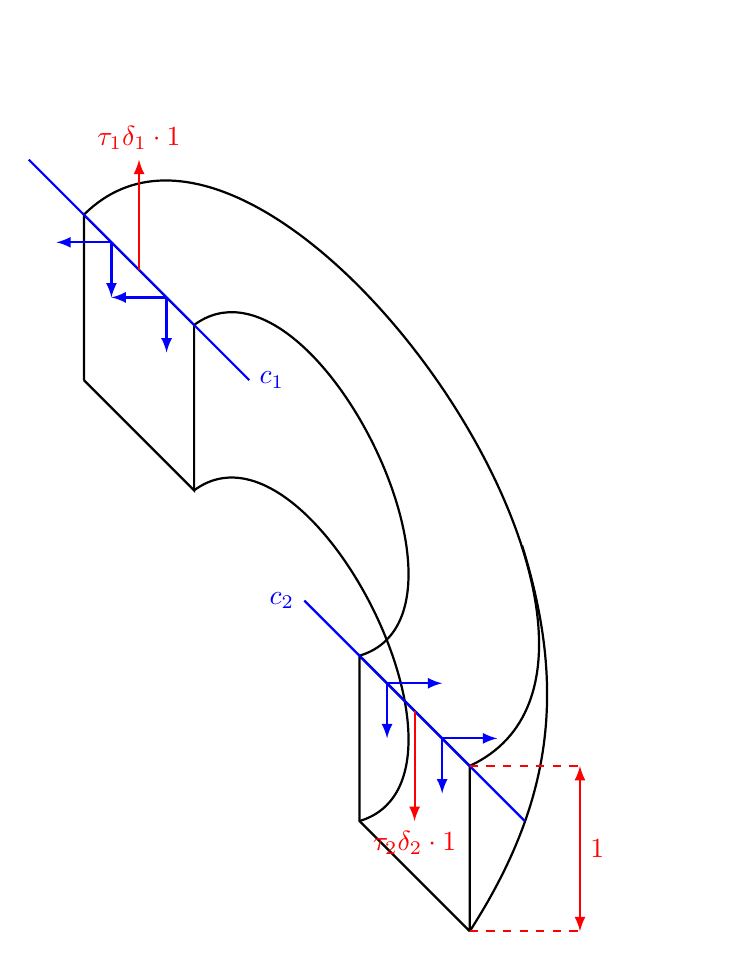
\begin{tikzpicture} [>=latex, scale=0.7]
			%		\draw [thin, help lines] (0,0) grid (15,15);
			%		\foreach \x in {0,...,15}
			%		\draw (\x cm,1pt) -- (\x cm,-1pt) node[anchor=north] {$\x$};
			%		\foreach \y in {0,...,15}
			%		\draw (1pt,\y cm) -- (-1pt,\y cm) node[anchor=east] {$\y$};
			%%% Solido
			\draw[thick] (1,11) -- (1,14) -- (3, 12) -- (3, 9) -- (1,11);
			\draw[thick] (8,1) -- (8,4) -- (6, 6) -- (6, 3) -- (8,1);	
			\draw[thick] (3,12) to[bend left = 100] (6,6);
			\draw[thick] (1,14) to[bend left = 100] (8,4);
			\draw[thick] (3,9) to[bend left = 100] (6,3);
			\draw[thick] (8.95,8) to[bend left=25] (8,1);
			%%% Corde
			\draw[thick, blue] (0,15) -- (4,11) node [pos = 1, right] {$c_1$};
			\draw[thick, blue] (5,7) -- (9,3) node [pos = 0, left] {$c_2$};
			%%% Vettori bassi
			\draw[->, thick, blue] (1.5,13.5) -- (1.5,12.5);
			\draw[->, thick, blue] (2.5,12.5) -- (2.5,11.5);
			%%% Vettori alti
			\draw[->, thick, blue] (1.5,13.5) -- (0.5,13.5);
			\draw[->, thick, blue] (2.5,12.5) -- (1.5,12.5);
			
			%%% Vettori bassi
			\draw[->, thick, blue] (6.5,5.5) -- (6.5,4.5);
			\draw[->, thick, blue] (7.5,4.5) -- (7.5,3.5);
			%%% Vettori alti
			\draw[->, thick, blue] (6.5,5.5) -- (7.5,5.5);
			\draw[->, thick, blue] (7.5,4.5) -- (8.5,4.5);
			%%% Vettori rossi
			\draw[->, thick, red] (2,13) -- (2,15) node [pos = 1, above] {$\tau_1\delta_1\cdot1$};
			\draw[->, thick, red] (7,5) -- (7,3) node [pos = 1, below] {$\tau_2\delta_2\cdot1$};
			%%% Dimensione 
			\draw[<->, thick, red] (10,1) -- (10,4) node [pos = 0.5, right] {1};
			\draw[dashed, thick, red] (8,4) -- (10,4);
			\draw[dashed, thick, red] (8,1) -- (10,1);	
		\end{tikzpicture}
	\end{center}
\end{figure}
		Se da una parte lo spessore cresce la tensione della parte opposta si riduce, in completa analogia idrodinamica, per una sezione stretta $\tau\uparrow$ mentre per una sezione larga $\tau\downarrow$: la tensione $\tau$ di dimostra così essere inversamente proporzionale allo spessore, al contrario delle sezioni aperte.\newline 
		
		Se si esprime l'equilibrio tra il momento torcente esterno e le azioni interne, questo diviene: 
		\[ M_0 = \oint_{l_m}\tau(s)\delta(s)h(s)ds = \tau(s)\delta(s)\oint_{l_m}h(s)ds = 0\]
		
\begin{figure}[H]
	\centering
	\label{fig:screenshot013}
	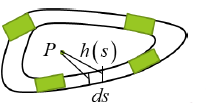
\includegraphics[width=0.5\linewidth]{immagini_5/screenshot013}
\end{figure}

		Dove $ h(s) $ è la distanza del polo dalla linea media, questa integrata sul percorso corrisponde proprio ad ottenere  il doppio dell'area sottesa dalla linea media stessa:
		\[{1\over2} \oint_{l_m}h(s)ds = \Omega_m \Rightarrow \oint_{l_m}h(s)ds = 2 \Omega_m\]
		E dunque l'equilibrio si può riscrivere: 
		\[ M_0 = \tau(s)\delta(s)\oint_{l_m}h(s)ds = \tau(s)\delta(s)2 \Omega_m = 0\]
		Giungendo infine a: 
		\[ \tau(s) = \dfrac{M_0}{2\delta(s) \Omega_m}\]
		Lo stato tensionale così ipotizzato prende il nome di tensioni alla
		Bredt. \newline 
		
		Si ricordi anche questa essere una soluzione approssimata,	questo valore infatti rappresenta l’aliquota costante della distribuzione legata ad un momento $M_0$. D'altro canto l'andamento è costante lungo lo spessore, ma in realtà l'andamento è questo: 
		
\begin{figure}[H]
	\centering
		\begin{tikzpicture} [>=latex]
	%%%	Help Lines
%	\draw [thin, help lines] (0,0) grid (5,5);
%	\foreach \x in {0,...,5}
%	\draw (\x cm,1pt) -- (\x cm,-1pt) node[anchor=north] {$\x$};
%	\foreach \y in {0,...,5}
%	\draw (1pt,\y cm) -- (-1pt,\y cm) node[anchor=east] {$\y$};
	%%%	Disegno	
	\draw (0, 2) -- (4,2);
	\draw (0, 1) -- (4,1);
	\draw[pattern = horizontal lines, ultra thick] (1,1) -- (1,2) -- (3,2) -- (3.25, 1) --(1,1);
	\draw[thin, red] (3,2) -- (3,1);
	\node at (2,2.25) {$M_0$};
	\node[red] at (3.5, 1.5) {$M_1$};
\end{tikzpicture}
\end{figure}

		È tuttavia una piccola variazione lungo lo spessore di cui si considera il solo contributo costante che darà un contributo a torsione pari ad $M_0$: l'andamento reale a farfalla è matematicamente trascurabile e posso confondere perciò $M_t \approx M_0$. 
		
		\[M_t = M_0 + M_1 \approx M_0\]
		
		Si è così dimostrato come la tensione tangenziale per questo tipo di sezioni sia inversamente proporzionale allo spessore della parete e all'area racchiusa dalla linea media. \newline 
		
		Questa formulazione è estremamente potente perché da un andamento delle tensioni molto semplificato, è però applicabile \underline{ESCLUSIVAMENTE} alle sezioni in parete sottile chiuse. 
